% Options for packages loaded elsewhere
\PassOptionsToPackage{unicode}{hyperref}
\PassOptionsToPackage{hyphens}{url}
%
\documentclass[
]{book}
\usepackage{lmodern}
\usepackage{amssymb,amsmath}
\usepackage{ifxetex,ifluatex}
\ifnum 0\ifxetex 1\fi\ifluatex 1\fi=0 % if pdftex
  \usepackage[T1]{fontenc}
  \usepackage[utf8]{inputenc}
  \usepackage{textcomp} % provide euro and other symbols
\else % if luatex or xetex
  \usepackage{unicode-math}
  \defaultfontfeatures{Scale=MatchLowercase}
  \defaultfontfeatures[\rmfamily]{Ligatures=TeX,Scale=1}
\fi
% Use upquote if available, for straight quotes in verbatim environments
\IfFileExists{upquote.sty}{\usepackage{upquote}}{}
\IfFileExists{microtype.sty}{% use microtype if available
  \usepackage[]{microtype}
  \UseMicrotypeSet[protrusion]{basicmath} % disable protrusion for tt fonts
}{}
\makeatletter
\@ifundefined{KOMAClassName}{% if non-KOMA class
  \IfFileExists{parskip.sty}{%
    \usepackage{parskip}
  }{% else
    \setlength{\parindent}{0pt}
    \setlength{\parskip}{6pt plus 2pt minus 1pt}}
}{% if KOMA class
  \KOMAoptions{parskip=half}}
\makeatother
\usepackage{xcolor}
\IfFileExists{xurl.sty}{\usepackage{xurl}}{} % add URL line breaks if available
\IfFileExists{bookmark.sty}{\usepackage{bookmark}}{\usepackage{hyperref}}
\hypersetup{
  pdftitle={PBR Notes},
  pdfauthor={Arden Rasmussen},
  hidelinks,
  pdfcreator={LaTeX via pandoc}}
\urlstyle{same} % disable monospaced font for URLs
\usepackage{longtable,booktabs}
% Correct order of tables after \paragraph or \subparagraph
\usepackage{etoolbox}
\makeatletter
\patchcmd\longtable{\par}{\if@noskipsec\mbox{}\fi\par}{}{}
\makeatother
% Allow footnotes in longtable head/foot
\IfFileExists{footnotehyper.sty}{\usepackage{footnotehyper}}{\usepackage{footnote}}
\makesavenoteenv{longtable}
\usepackage{graphicx,grffile}
\makeatletter
\def\maxwidth{\ifdim\Gin@nat@width>\linewidth\linewidth\else\Gin@nat@width\fi}
\def\maxheight{\ifdim\Gin@nat@height>\textheight\textheight\else\Gin@nat@height\fi}
\makeatother
% Scale images if necessary, so that they will not overflow the page
% margins by default, and it is still possible to overwrite the defaults
% using explicit options in \includegraphics[width, height, ...]{}
\setkeys{Gin}{width=\maxwidth,height=\maxheight,keepaspectratio}
% Set default figure placement to htbp
\makeatletter
\def\fps@figure{htbp}
\makeatother
\setlength{\emergencystretch}{3em} % prevent overfull lines
\providecommand{\tightlist}{%
  \setlength{\itemsep}{0pt}\setlength{\parskip}{0pt}}
\setcounter{secnumdepth}{5}

\title{PBR Notes}
\author{Arden Rasmussen}
\date{}

\begin{document}
\frontmatter
\maketitle

{
\setcounter{tocdepth}{2}
\tableofcontents
}
\mainmatter
\hypertarget{tu-wien-rendering}{%
\chapter{TU Wien Rendering}\label{tu-wien-rendering}}

\hypertarget{radiometry-recap-light-attenuation}{%
\chapter{Radiometry Recap, Light Attenuation}\label{radiometry-recap-light-attenuation}}

\hypertarget{radiometry-recap}{%
\section{Radiometry Recap}\label{radiometry-recap}}

\textbf{What to measure in a simulation?}

\begin{description}
\tightlist
\item[Radiant flux (or power)]
Total amount of energy passing through a surface (measured per second).
\[ \Phi \left[W\right]\]
\end{description}

It is not good to measurethe radiant flux , because it is the energy per
surface, so a large radiant flux could either be

\begin{enumerate}
\def\labelenumi{\arabic{enumi}.}
\tightlist
\item
  A lot of energy over a small surface.
\item
  A little energy over a large surface.
\end{enumerate}

This metric is ambiguious, and thus it is not good enough.

Lets comput the flux by unit area (irradiance).
\[E\left[W/m^2\right]\]

This is still ambiguous, we haven't fixed the angle wihc the ligh arives to the
surface. So

\begin{enumerate}
\def\labelenumi{\arabic{enumi}.}
\tightlist
\item
  A lot of energy in a huge angle.
\item
  A little energy in a small angle.
\end{enumerate}

will measure the same irradiance.

Compute the flux by unit area and unit angle(radiance).
\[L\left[W/\left(m^2\cdot sr\right)\right]\]

\emph{Note:} angle in more diemsions is called solid angle, for which the unit is
steradians.

This is the measurement that we will be using to measure.

\hypertarget{the-most-fundamental-question}{%
\section{The most fundamental question}\label{the-most-fundamental-question}}

\textbf{How much light exiss a surface point in a given direction?}

The answer is given by Maxwell equations!

In practice, we don't do this, it would be too complicated.

The real solution is the rendering equation!

\hypertarget{the-scalar-product}{%
\section{The scalar product}\label{the-scalar-product}}

\[
\vec{a}\cdot\vec{b}\equiv||\vec{a}||\cdot||\vec{b}||\cos\theta
\]

We will usualy use vectors of unit length, so
\[
\vec{a}\cdot\vec{b}\equiv\cos\theta
\]

\hypertarget{terminology}{%
\section{Terminology}\label{terminology}}

\begin{figure}
\centering
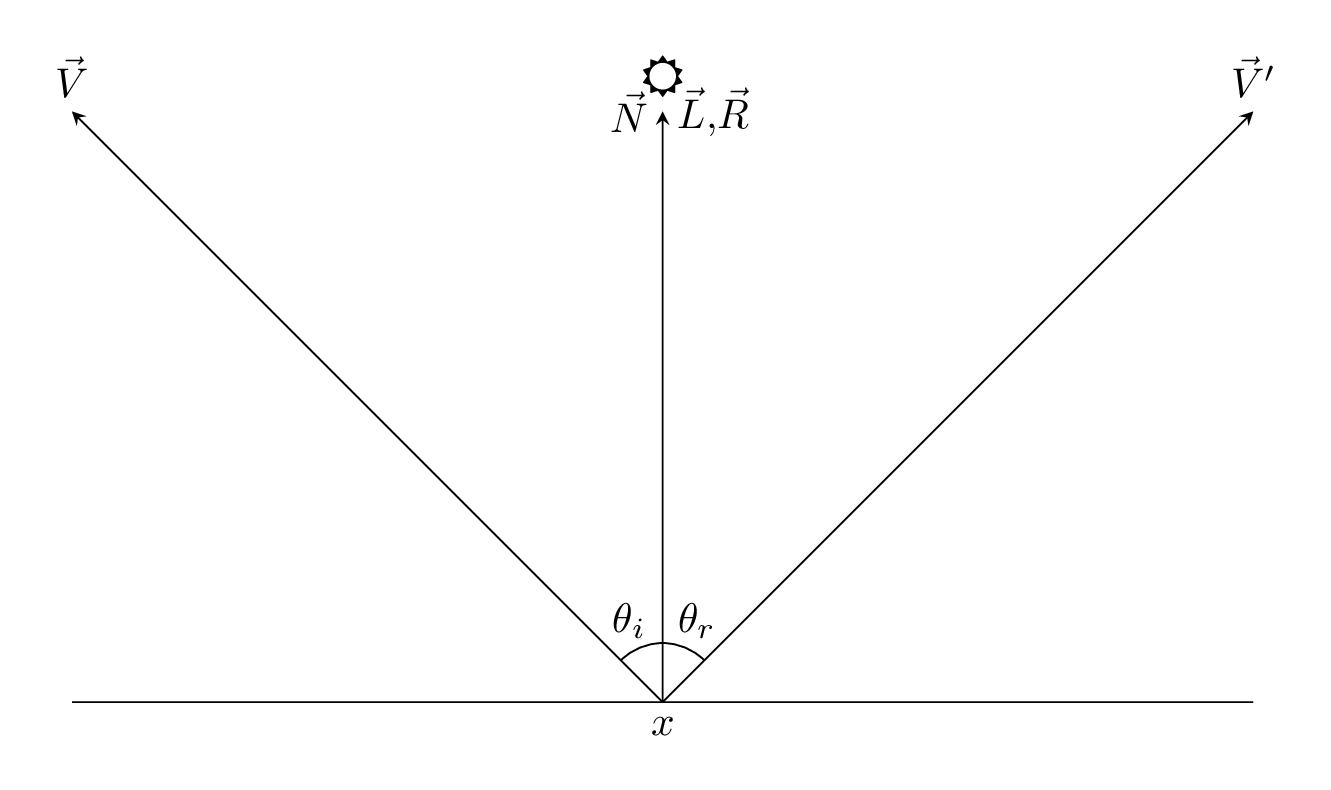
\includegraphics{figures/02_1.png}
\caption{Figure}
\end{figure}

\begin{itemize}
\tightlist
\item
  \(\vec{V}\) direction towards the viewer (eye,camera)
\item
  \(\vec{N}\) surface normal
\item
  \(\vec{L}\) vector point towards the light source
\item
  \(\vec{R}\) reflected ray direction
  \(\vec{R}=\vec{L}-2\vec{N}\left(\vec{L}\cdot\vec{N}\right)\).
\item
  \(\theta_i,\theta_r\) incident and reflected angles
\end{itemize}

Vectors are always pointing out form the point \(x\).

\hypertarget{light-attenuation}{%
\section{Light Attenuation}\label{light-attenuation}}

When the sun is directly above as in the prvious figure.
\[
\left(\vec{L}\cdot\vec{N}\right)\Phi=\cos0\Phi=\Phi
\]

If the sun is off to one side as in this figure if \(\alpha\approx45^\circ\).

\begin{figure}
\centering
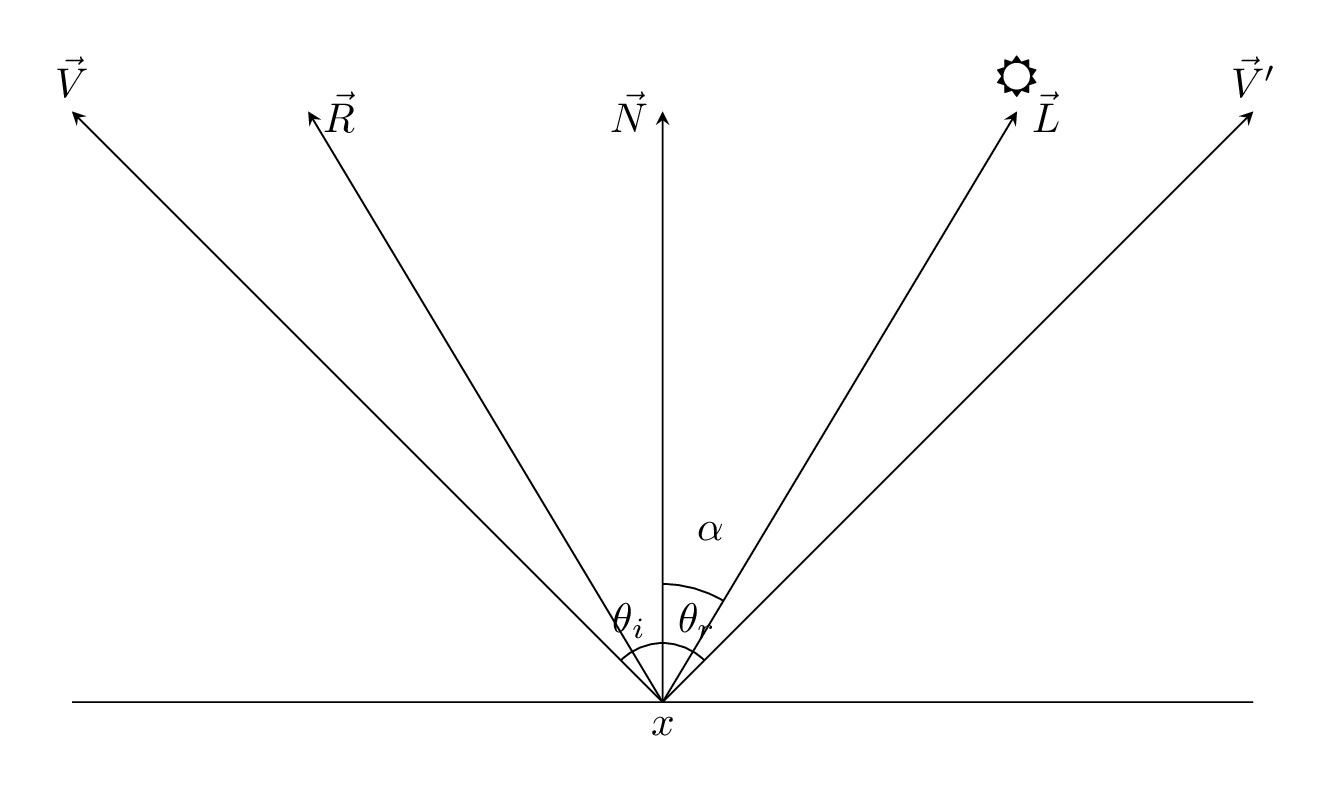
\includegraphics{figures/02_2.png}
\caption{Figure}
\end{figure}

\[
\left(\vec{L}\cdot\vec{N}\right)\Phi=\cos\alpha\Phi\approx 0.7\Phi
\]

If the sun is near \(90^\circ\), as in this figure, where
\(\alpha\approx90^\circ\).

\begin{figure}
\centering
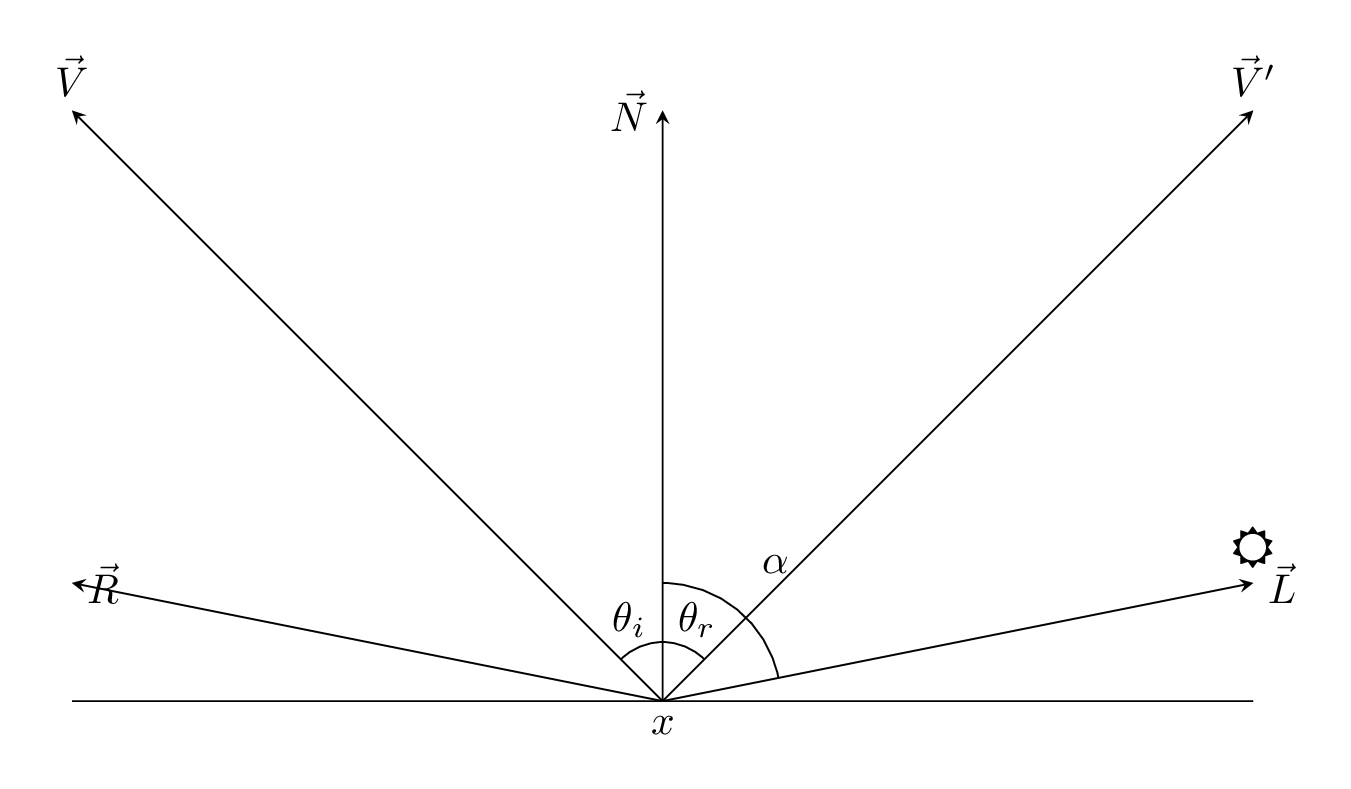
\includegraphics{figures/02_3.png}
\caption{Figure}
\end{figure}

\[
\left(\vec{L}\cdot\vec{N}\right)\Phi=\cos\alpha\Phi\approx 0
\]

Thus we can model the light attenuation using this dot product.

\backmatter
\end{document}
